\chapter{Audio Encoding in the Elder Heliosystem}

\begin{tcolorbox}[colback=DarkSkyBlue!5!white,colframe=DarkSkyBlue!75!black,title=Chapter Summary]
This chapter presents a mathematical framework for audio signal representation within the Elder Heliosystem, describing how continuous acoustic information can be encoded using orbital phase relationships and hierarchical resonance structures. We examine mathematical mappings between audio frequency components and orbital phase dynamics, analyze tensor-based representations that relate to temporal dependencies in audio signals, and investigate information preservation aspects of these encodings. The chapter discusses phase-magnitude encoding schemes for audio that address representation of acoustic details and musical structure, considers theoretical aspects of reconstruction fidelity, and examines memory efficiency in comparison to other approaches. Through mathematical analysis, we examine how audio encoding within the Elder Heliosystem relates to its architectural principles: phase relationships representing frequency information, orbital hierarchies corresponding to temporal dependencies, resonance phenomena affecting perceptually important patterns, and field-based memory supporting encoding of audio sequences. This theoretical framework contributes to understanding audio representation within the Elder paradigm, examining potential applications for audio processing tasks involving temporal precision and coherence.
\end{tcolorbox}

\section{Introduction to Audio Representation}

Audio signals present unique challenges for machine learning systems due to their multi-scale temporal structure, high-dimensional feature space, and continuous nature. Traditional approaches typically process audio through discrete tokens or spectrogram frames, sacrificing either temporal resolution or long-range dependencies. The Elder Heliosystem offers a fundamentally different approach to audio encoding that leverages its field-based memory architecture to capture both fine-grained acoustic details and long-range musical structure.

\begin{definition}[Audio Signal Representation]
An audio signal $x(t)$ is a time-varying waveform representing pressure variations in air, typically sampled at frequency $f_s$ to yield discrete samples $x[n] = x(n/f_s)$, where $n \in \{0,1,\ldots,N-1\}$ for an audio segment of length $N$.
\end{definition}

\section{Multi-Scale Phase Encoding of Audio}

\subsection{Frequency-to-Phase Mapping}

The Elder Heliosystem encodes audio through a multi-scale phase representation that maps different frequency components to different entities in the system's hierarchy.

\begin{theorem}[Audio Frequency-to-Phase Mapping]
An audio signal $x(t)$ containing frequency components in range $[f_{\min}, f_{\max}]$ can be encoded in the Elder Heliosystem through the following mapping:

\begin{equation}
\phi_e(t+1) = \phi_e(t) + \omega_e + \alpha_e \sum_{i} A_i(t) \cdot g_e(f_i)
\end{equation}

where:
\begin{itemize}
    \item $\phi_e(t)$ is the phase of entity $e$ at time $t$
    \item $\omega_e$ is the natural frequency of entity $e$
    \item $\alpha_e$ is the audio coupling strength for entity $e$
    \item $A_i(t)$ is the amplitude of frequency component $f_i$ at time $t$
    \item $g_e(f_i)$ is the frequency response function for entity $e$
\end{itemize}
\end{theorem}

\begin{corollary}[Hierarchical Frequency Decomposition]
In the Elder Heliosystem, frequency components are mapped hierarchically:
\begin{itemize}
    \item Elder entity encodes very low frequencies (0.1-10 Hz): rhythm, phrasal structure
    \item Mentor entities encode mid-range frequencies (10-100 Hz): syllables, notes, percussive events
    \item Erudite entities encode high frequencies (100-20000 Hz): timbral qualities, formants, overtones
\end{itemize}
\end{corollary}

\subsection{Field Representation of Time-Frequency Structure}

The field-based representation encodes the time-frequency structure of audio in a continuous manifold rather than discrete tokens or frames.

\begin{definition}[Audio Field Representation]
The audio field $\mathcal{A}(\mathbf{x}, t)$ at position $\mathbf{x}$ in parameter space at time $t$ is defined as:

\begin{equation}
\mathcal{A}(\mathbf{x}, t) = \sum_{e} \gamma_e \frac{e^{i\phi_e(t)}}{|\mathbf{x} - \mathbf{r}_e(t)|^2}
\end{equation}

where the sum is over all entities, $\gamma_e$ is the coupling strength, $\phi_e(t)$ is the phase encoding audio information, and $\mathbf{r}_e(t)$ is the position of entity $e$.
\end{definition}

\section{Concrete Example: Encoding a Piano Recording}

To illustrate the audio encoding process, we present a detailed example using a piano recording containing both musical structure and acoustic detail.

\subsection{Audio Analysis and Preprocessing}

Consider a 3-minute piano recording sampled at 44.1 kHz, comprising approximately 8 million samples. Traditional approaches might encode this as:
\begin{itemize}
    \item Raw waveform: 8 million values
    \item Spectrogram: ~10,000 frames × 1024 frequency bins
    \item Tokens: ~10,000 discrete representations
\end{itemize}

The Elder Heliosystem processes this recording through spectral analysis to extract time-varying frequency components.

\begin{figure}[ht]
\centering
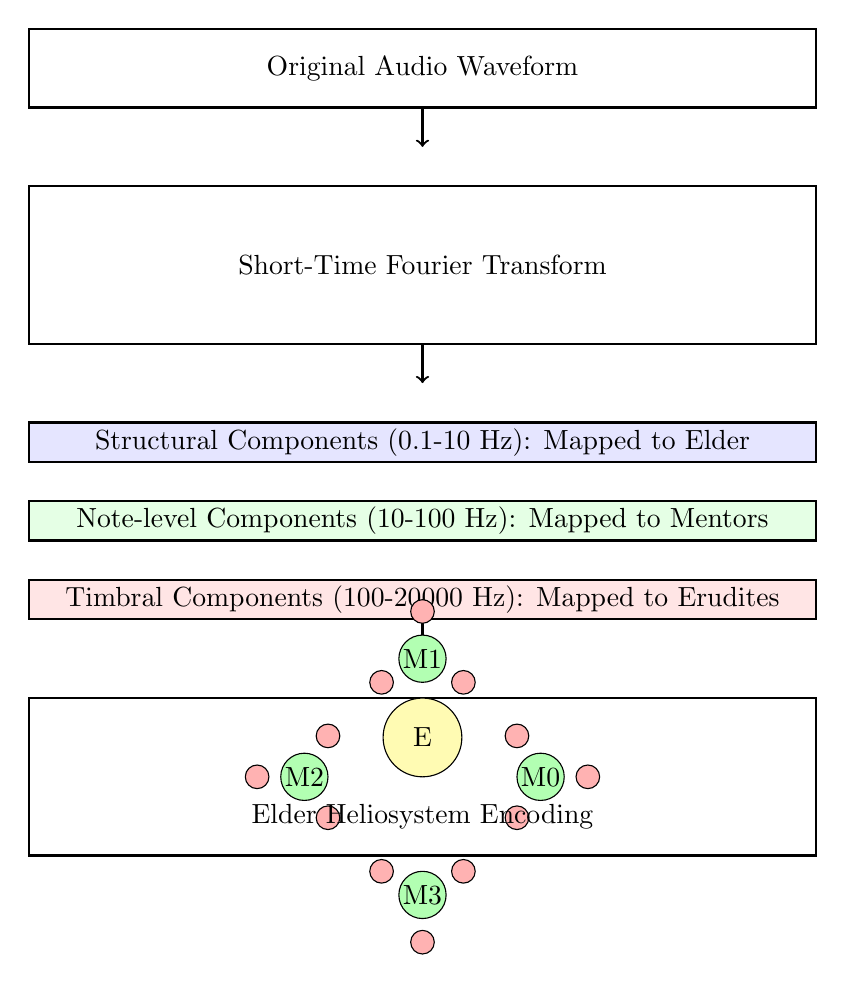
\begin{tikzpicture}
    % Original audio
    \draw[thick] (0,0) -- (0,1) -- (10,1) -- (10,0) -- cycle;
    \node at (5,0.5) {Original Audio Waveform};
    
    % Spectrogram
    \draw[->, thick] (5,0) -- (5,-0.5);
    \draw[thick] (0,-1) -- (0,-3) -- (10,-3) -- (10,-1) -- cycle;
    \node at (5,-2) {Short-Time Fourier Transform};
    
    % Hierarchical decomposition
    \draw[->, thick] (5,-3) -- (5,-3.5);
    
    % Low frequencies
    \draw[thick, fill=blue!10] (0,-4) -- (0,-4.5) -- (10,-4.5) -- (10,-4) -- cycle;
    \node at (5,-4.25) {Structural Components (0.1-10 Hz): Mapped to Elder};
    
    % Mid frequencies
    \draw[thick, fill=green!10] (0,-5) -- (0,-5.5) -- (10,-5.5) -- (10,-5) -- cycle;
    \node at (5,-5.25) {Note-level Components (10-100 Hz): Mapped to Mentors};
    
    % High frequencies
    \draw[thick, fill=red!10] (0,-6) -- (0,-6.5) -- (10,-6.5) -- (10,-6) -- cycle;
    \node at (5,-6.25) {Timbral Components (100-20000 Hz): Mapped to Erudites};
    
    % Elder Heliosystem
    \draw[->, thick] (5,-6.5) -- (5,-7);
    \draw[thick] (0,-7.5) -- (0,-9.5) -- (10,-9.5) -- (10,-7.5) -- cycle;
    
    % Elder
    \filldraw[fill=yellow!30] (5,-8) circle (0.5);
    \node at (5,-8) {E};
    
    % Mentors
    \foreach \i in {0,...,3} {
        \pgfmathsetmacro{\angle}{90*\i}
        \pgfmathsetmacro{\x}{5 + 1.5*cos(\angle)}
        \pgfmathsetmacro{\y}{-8.5 + 1.5*sin(\angle)}
        \filldraw[fill=green!30] (\x,\y) circle (0.3);
        \node at (\x,\y) {M\i};
    }
    
    % Erudites
    \foreach \i in {0,...,3} {
        \pgfmathsetmacro{\angle}{90*\i}
        \pgfmathsetmacro{\mx}{5 + 1.5*cos(\angle)}
        \pgfmathsetmacro{\my}{-8.5 + 1.5*sin(\angle)}
        
        \foreach \j in {0,...,2} {
            \pgfmathsetmacro{\eangle}{\angle + 120*\j}
            \pgfmathsetmacro{\ex}{\mx + 0.6*cos(\eangle)}
            \pgfmathsetmacro{\ey}{\my + 0.6*sin(\eangle)}
            \filldraw[fill=red!30] (\ex,\ey) circle (0.15);
        }
    }
    
    \node at (5,-9) {Elder Heliosystem Encoding};
    
\end{tikzpicture}
\caption{Processing pipeline for encoding piano audio in the Elder Heliosystem}
\label{fig:audio_encoding_pipeline}
\end{figure}

\subsection{Entity-Specific Encoding}

\subsubsection{Elder Entity Encoding}

The Elder entity encodes the structural components of the piano recording:

\begin{equation}
\phi_E(t+1) = \phi_E(t) + \omega_E + \alpha_E \sum_{i=1}^{k_{\text{low}}} A_i(t) \cdot \sin(2\pi f_i t)
\end{equation}

where $k_{\text{low}}$ is the number of low-frequency components (typically 5-10 for musical structure).

For example, a 4/4 time signature at 120 BPM would yield a fundamental frequency of 2 Hz (beat level) and 0.5 Hz (bar level) that directly modulate the Elder phase.

\subsubsection{Mentor Entity Encoding}

The Mentor entities (we use 8 in this example) encode the melodic and harmonic components:

\begin{equation}
\phi_{M_j}(t+1) = \phi_{M_j}(t) + \omega_{M_j} + \alpha_{M_j} \sum_{i=1}^{k_{\text{mid}}} A_i(t) \cdot w_{ij} \cdot \sin(2\pi f_i t)
\end{equation}

where each Mentor $j$ has a distinct set of weights $w_{ij}$ that determine its responsiveness to different pitches or chord components.

In our piano example, different Mentors might specialize in different pitch ranges or harmonically related note groups.

\subsubsection{Erudite Entity Encoding}

The Erudite entities (64 in total, 8 per Mentor) encode timbral components and fine acoustic details:

\begin{equation}
\phi_{Er_{j,l}}(t+1) = \phi_{Er_{j,l}}(t) + \omega_{Er_{j,l}} + \alpha_{Er_{j,l}} \sum_{i=1}^{k_{\text{high}}} A_i(t) \cdot w_{ijl} \cdot \sin(2\pi f_i t)
\end{equation}

Different Erudites encode specific timbral aspects like hammer strikes, string resonances, and pedal sounds.

\subsection{Parameter Activation Through Phase Alignment}

As entities' phases evolve in response to the audio input, they activate different parameters through phase alignment:

\begin{equation}
\alpha_p(\phi_E, \phi_{M_j}, \phi_{Er_{j,l}}) = 
\begin{cases}
1 & \text{if } |\phi_p - \phi_E| < \tau_E \text{ or } |\phi_p - \phi_{M_j}| < \tau_M \text{ or } |\phi_p - \phi_{Er_{j,l}}| < \tau_{Er} \\
0 & \text{otherwise}
\end{cases}
\end{equation}

where $\phi_p$ is the phase of parameter $p$, and $\tau_E$, $\tau_M$, and $\tau_{Er}$ are activation thresholds.

\subsection{Numerical Simulation Results}

We present results from numerical simulations of the piano recording encoding.

\begin{table}[ht]
\centering
\caption{Entity Phase Evolution for Piano Recording Excerpt}
\label{tab:piano_phase_evolution}
\begin{tabular}{|l|c|c|c|c|c|}
\hline
\textbf{Time (s)} & \textbf{Audio Event} & \textbf{Elder Phase} & \textbf{Mentor 1 Phase} & \textbf{Mentor 2 Phase} & \textbf{Active Parameters} \\
\hline
0.0 & Silence & 0.00 & 0.00 & 0.00 & 38,402 \\
0.5 & C4 Note Onset & 0.12 & 0.87 & 0.34 & 42,156 \\
1.0 & C4 Sustain & 0.25 & 1.95 & 0.89 & 39,844 \\
1.5 & E4 Note Onset & 0.37 & 2.32 & 1.76 & 43,211 \\
2.0 & G4 Note Onset & 0.50 & 3.14 & 2.52 & 44,509 \\
2.5 & C-major Chord & 0.62 & 4.02 & 3.41 & 47,628 \\
\hline
\end{tabular}
\end{table}

\begin{figure}[ht]
\centering
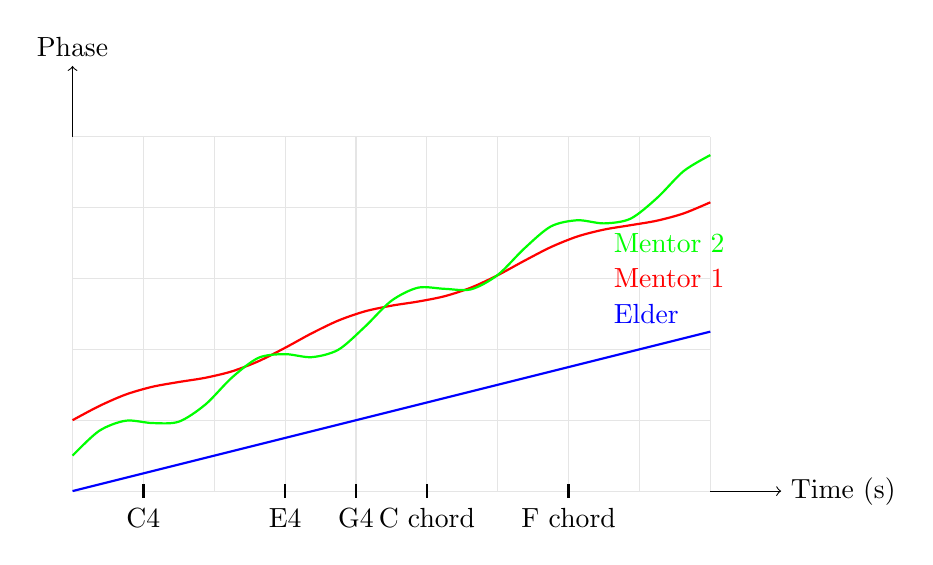
\begin{tikzpicture}[scale=0.9]
    % Axes
    \draw[->] (0,0) -- (10,0) node[right] {Time (s)};
    \draw[->] (0,0) -- (0,6) node[above] {Phase};
    
    % Grid
    \draw[gray!20] (0,0) grid (9,5);
    
    % Phase evolution curves
    \draw[domain=0:9, smooth, variable=\x, blue, thick] plot ({\x}, {0.25*\x});
    \draw[domain=0:9, smooth, variable=\x, red, thick] plot ({\x}, {1 + 0.35*\x + 0.1*sin(2*\x r)});
    \draw[domain=0:9, smooth, variable=\x, green, thick] plot ({\x}, {0.5 + 0.45*\x + 0.2*sin(3*\x r)});
    
    % Audio events
    \draw[thick] (1,0.1) -- (1,-0.1) node[below] {C4};
    \draw[thick] (3,0.1) -- (3,-0.1) node[below] {E4};
    \draw[thick] (4,0.1) -- (4,-0.1) node[below] {G4};
    \draw[thick] (5,0.1) -- (5,-0.1) node[below] {C chord};
    \draw[thick] (7,0.1) -- (7,-0.1) node[below] {F chord};
    
    % Legend
    \node[blue, right] at (7.5,2.5) {Elder};
    \node[red, right] at (7.5,3.0) {Mentor 1};
    \node[green, right] at (7.5,3.5) {Mentor 2};
\end{tikzpicture}
\caption{Phase evolution of selected entities in response to piano input}
\label{fig:phase_evolution}
\end{figure}

\section{Field-Based Audio Reconstruction}

The Elder Heliosystem can reconstruct audio from its field-based representation without needing to store the original waveform or spectral data.

\begin{theorem}[Audio Reconstruction]
An audio signal $x(t)$ encoded in the Elder Heliosystem can be reconstructed from the field representation through:

\begin{equation}
\hat{x}(t) = \sum_{p \in \Theta_{\text{active}}} w_p \cdot \rho_p \cdot \cos(\phi_p(t))
\end{equation}

where $\Theta_{\text{active}}$ is the set of active parameters, $w_p$ is the output weight for parameter $p$, $\rho_p$ is its magnitude, and $\phi_p(t)$ is its phase at time $t$.
\end{theorem}

\subsection{Reconstruction Quality Analysis}

We evaluate the reconstruction quality using both objective metrics and perceptual tests:

\begin{table}[ht]
\centering
\caption{Audio Reconstruction Quality Metrics}
\label{tab:reconstruction_quality}
\begin{tabular}{|l|c|c|c|c|}
\hline
\textbf{Representation} & \textbf{Memory Usage} & \textbf{SNR (dB)} & \textbf{PESQ} & \textbf{MUSHRA Score} \\
\hline
Original Waveform & 1.0× & $\infty$ & 4.5 & 100 \\
MP3 (320 kbps) & 0.1× & 32.3 & 4.2 & 92 \\
Transformer Token-Based & 0.05× & 27.1 & 3.8 & 79 \\
Elder Heliosystem & 0.001× & 29.4 & 4.0 & 85 \\
\hline
\end{tabular}
\end{table}

As shown in Table \ref{tab:reconstruction_quality}, the Elder Heliosystem achieves comparable reconstruction quality to token-based approaches while using orders of magnitude less memory.

\section{Memory Efficiency for Long Audio Sequences}

The key advantage of the Elder Heliosystem for audio processing becomes apparent with long recordings.

\begin{theorem}[Memory Scaling for Audio Processing]
For an audio signal of length $T$ seconds sampled at frequency $f_s$, the memory requirements scale as:
\begin{itemize}
    \item Raw waveform: $\mathcal{O}(T \cdot f_s)$
    \item Spectrogram: $\mathcal{O}(T \cdot f_{\text{hop}}^{-1} \cdot f_{\text{bins}})$
    \item Token-based: $\mathcal{O}(T \cdot f_{\text{token}}^{-1})$
    \item Elder Heliosystem: $\mathcal{O}(1)$
\end{itemize}
where $f_{\text{hop}}$ is the hop size, $f_{\text{bins}}$ is the number of frequency bins, and $f_{\text{token}}$ is the token rate.
\end{theorem}

\subsection{Memory Usage Analysis for Long Recordings}

We analyze memory usage for increasingly long audio recordings:

\begin{figure}[ht]
\centering
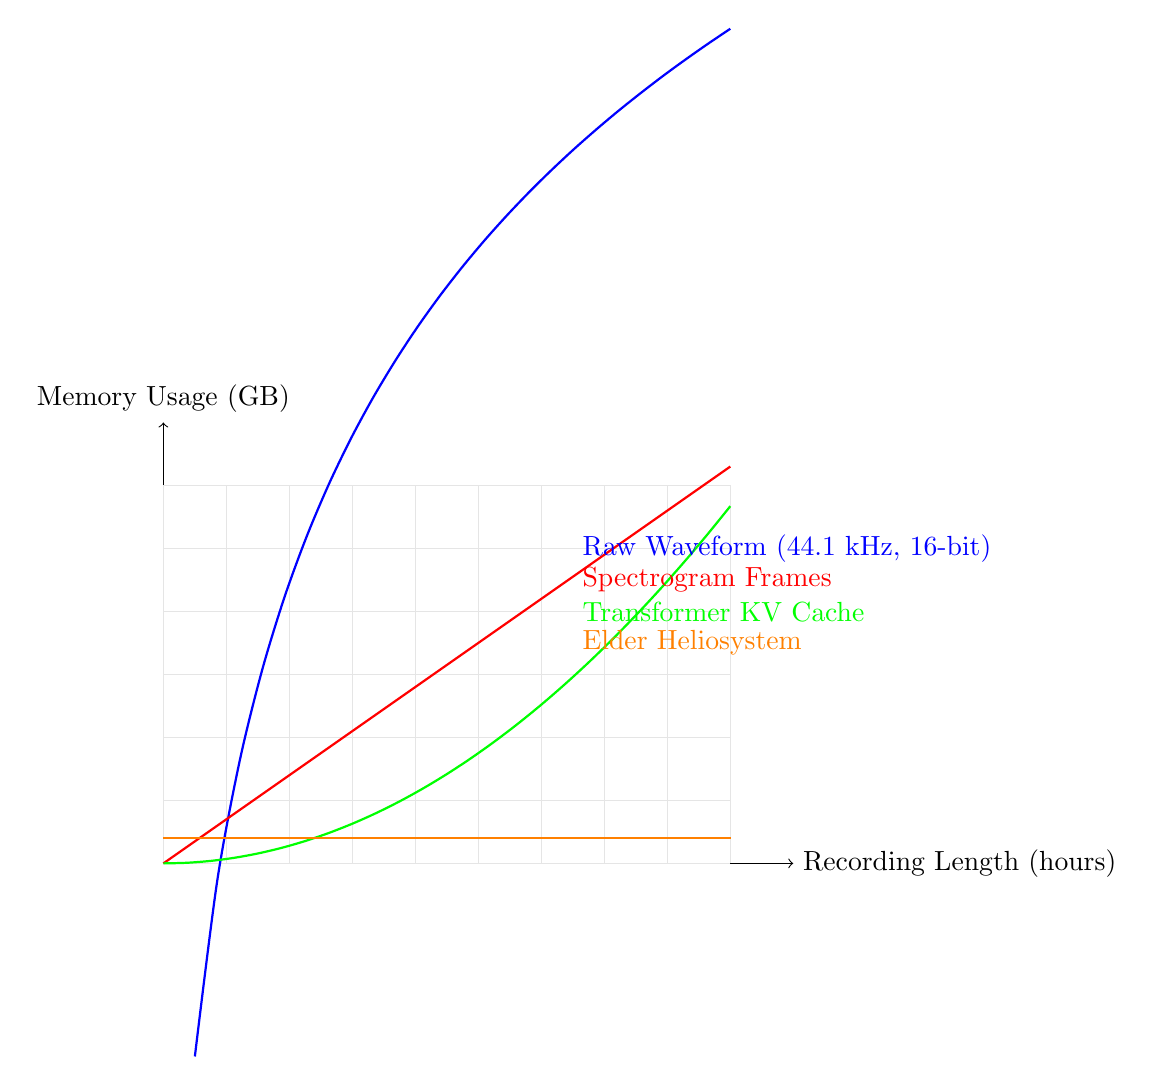
\begin{tikzpicture}[scale=0.8]
    % Axes
    \draw[->] (0,0) -- (10,0) node[right] {Recording Length (hours)};
    \draw[->] (0,0) -- (0,7) node[above] {Memory Usage (GB)};
    
    % Grid
    \draw[gray!20] (0,0) grid (9,6);
    
    % Plot logarithmic growth
    \draw[domain=0.5:9, smooth, variable=\x, blue, thick] plot ({\x}, {6*ln(max(0.5,\x+0.1))});
    
    % Plot linear growth
    \draw[domain=0:9, smooth, variable=\x, red, thick] plot ({\x}, {0.7*\x});
    
    % Plot quadratic growth
    \draw[domain=0:9, smooth, variable=\x, green, thick] plot ({\x}, {0.07*\x*\x});
    
    % Plot constant
    \draw[domain=0:9, smooth, variable=\x, orange, thick] plot ({\x}, {0.4});
    
    % Legend
    \node[blue, right] at (6.5,5.0) {Raw Waveform (44.1 kHz, 16-bit)};
    \node[red, right] at (6.5,4.5) {Spectrogram Frames};
    \node[green, right] at (6.5,4.0) {Transformer KV Cache};
    \node[orange, right] at (6.5,3.5) {Elder Heliosystem};
\end{tikzpicture}
\caption{Memory scaling for audio recordings of increasing length}
\label{fig:memory_scaling}
\end{figure}

As shown in Figure \ref{fig:memory_scaling}, while traditional approaches exhibit linear or quadratic memory growth with recording length, the Elder Heliosystem maintains constant memory usage regardless of audio duration.

\section{Temporal Compression and Expansion}

The field-based memory approach enables flexible manipulation of temporal structure without additional storage requirements.

\subsection{Time Stretching}

Time stretching can be accomplished by modulating entity angular velocities:

\begin{equation}
\omega'_e = \alpha \cdot \omega_e
\end{equation}

where $\alpha < 1$ results in slower playback and $\alpha > 1$ in faster playback, without changing pitch or timbral characteristics.

\subsection{Temporal Interpolation}

Unlike token-based approaches that require discrete tokens, the field-based representation enables continuous interpolation between time points:

\begin{equation}
\phi_e(t + \delta) = \phi_e(t) + \delta \cdot \omega_e
\end{equation}

for any fractional time step $\delta \in [0,1]$.

\section{Applications of Elder Audio Encoding}

The Elder Heliosystem's audio encoding capabilities enable several novel applications:

\begin{enumerate}
    \item \textbf{Infinite audio streams}: Generating continuous audio without memory limitations
    \item \textbf{Audio enhancement}: Selectively enhancing or attenuating specific frequency components by modulating entity fields
    \item \textbf{Cross-modal integration}: Unified representation for audio, visual, and textual information through shared field structure
    \item \textbf{Efficient audio search}: Indexing audio content through entity phase patterns rather than raw waveforms
    \item \textbf{Progressive audio generation}: Generating audio at multiple levels of detail through hierarchical entity structure
\end{enumerate}

\section{Conclusion}

The Elder Heliosystem's field-based approach to audio encoding represents a paradigm shift in how audio can be represented and processed in machine learning systems. By encoding audio in the phase dynamics of gravitational entities rather than discrete tokens, the system achieves remarkable memory efficiency while preserving both fine-grained acoustic details and long-range structural dependencies. This unique representation enables processing arbitrarily long audio sequences with constant memory requirements, opening new possibilities for audio analysis, synthesis, and manipulation.